% =============================================================================
% main.tex - Master Document
% scRNA-seq Clustering Comparative Study
% =============================================================================

\documentclass[11pt,a4paper]{article}

% =============================================================================
% preamble.tex - LaTeX Preamble for scRNA-seq Clustering Study
% =============================================================================

% Document setup
\usepackage[utf8]{inputenc}
\usepackage[T1]{fontenc}
\usepackage[english]{babel}

% Page geometry
\usepackage[a4paper, margin=2.5cm]{geometry}

% Headers and footers
\usepackage{fancyhdr}
\pagestyle{fancy}
\fancyhf{} % Clear all headers and footers

% Adjust header height and compensate top margin
\setlength{\headheight}{32.54pt}
\addtolength{\topmargin}{-20.54pt}

% Add image to header (centered) - using width for better proportions
\fancyhead[C]{
\includegraphics[width=0.5\textwidth]{figures/logo.jpg}}
% Adjust width as needed: 0.2\textwidth (narrow), 0.3\textwidth (medium), 0.4\textwidth (wide)

% Add page numbers to footer
\fancyfoot[C]{\thepage}

% Customize header rule thickness
\renewcommand{\headrulewidth}{0.4pt}

% Math packages
\usepackage{amsmath}
\usepackage{amssymb}
\usepackage{amsthm}

% Graphics and figures
\usepackage{graphicx}
\usepackage{float}
\usepackage{subcaption}

% Tables
\usepackage{booktabs}
\usepackage{multirow}
\usepackage{longtable}

% Colors
\usepackage{xcolor}
\definecolor{codeblue}{RGB}{0, 102, 204}
\definecolor{codegray}{RGB}{128, 128, 128}

% Hyperlinks
\usepackage[colorlinks=true, linkcolor=blue, citecolor=blue, urlcolor=codeblue]{hyperref}

% Bibliography
\usepackage[numbers,sort&compress]{natbib}

% Code listings
\usepackage{listings}
\lstset{
    basicstyle=\ttfamily\small,
    keywordstyle=\color{codeblue},
    commentstyle=\color{codegray},
    breaklines=true,
    frame=single,
    numbers=left,
    numberstyle=\tiny\color{codegray}
}

% Algorithms
\usepackage{algorithm}
\usepackage{algpseudocode}

% Misc
\usepackage{enumitem}
\usepackage{url}
\usepackage{microtype}

% Custom commands
\newcommand{\ari}{\text{ARI}}
\newcommand{\nmi}{\text{NMI}}
\newcommand{\fdp}{\text{FDP}}
\newcommand{\fdr}{\text{FDR}}

% Theorems and definitions
\theoremstyle{definition}
\newtheorem{definition}{Definition}[section]


% Document metadata
\title{A Comparative Study of Statistical Calibration Methods\\for Single-Cell RNA Sequencing Clustering}
\author{
    Stanea Adrian-Bogdan\\
    \textit{Technical University of Cluj-Napoca}\\
    \texttt{adrianstanea1@gmail.com}
}
\date{\today}

% =============================================================================
\begin{document}
% =============================================================================

\maketitle

\newpage
% Abstract
% =============================================================================
% 00_abstract.tex - Abstract
% =============================================================================

\begin{abstract}

Single-cell RNA sequencing (scRNA-seq) has revolutionized our understanding of cellular heterogeneity, yet the identification of distinct cell populations through clustering remains a significant challenge. Current graph-based clustering methods, such as Leiden and Louvain, rely heavily on user-defined resolution parameters, leading to reproducibility issues and the risk of over-clustering or under-clustering. Additionally, the common practice of performing differential expression analysis on the same data used for clustering---known as ``double-dipping''---inflates false discovery rates and produces spurious cell type markers.

In this study, we present a comparative analysis of clustering methods designed to address these limitations. We evaluate three approaches: (1) \textbf{Seurat/Leiden}, the standard graph-based community detection method at multiple resolution parameters; (2) \textbf{SC3} (Single-Cell Consensus Clustering), which employs an ensemble of k-means clusterings with spectral dimensionality reduction and automatic $k$ estimation; and (3) \textbf{recall}, which uses knockoff variables to control the false discovery rate during cluster calibration. We benchmark these methods on three datasets with known ground truth: scMixology (902 cells, 3 cell lines), PBMC 3k (2,643 cells, 9 cell types), and Zeisel mouse brain (680 cells, 7 neuronal classes).

Our results demonstrate that Leiden clustering at low resolution (0.2) achieves the highest accuracy on the scMixology dataset (ARI = 0.856), followed by SC3 (ARI = 0.741) and recall (ARI = 0.680). On the more complex PBMC 3k dataset, Leiden at resolution 1.0 achieves ARI = 0.781, while recall maintains competitive performance (ARI = 0.649). SC3 encountered memory constraints on larger datasets, highlighting scalability considerations for consensus-based methods.

\vspace{1em}
\noindent\textbf{Keywords:} single-cell RNA-seq, clustering, SC3, recall, Leiden, knockoff variables, consensus clustering, reproducibility

\end{abstract}


\newpage
% Table of contents (optional)
\tableofcontents
\newpage

% Main sections
% =============================================================================
% 01_introduction.tex - Introduction
% =============================================================================

\section{Introduction}
\label{sec:introduction}

\subsection{The Evolution of Cell Type Discovery}

The identification of cell types from transcriptomic data has undergone significant evolution over the past decade. Early methods (2013--2016) relied on distance-based metrics and k-means clustering, which assumed spherical cluster shapes---an assumption rarely met in the complex, continuous manifolds of biological development~\cite{kiselev2019challenges}. Among these early methods, SC3 (Single-Cell Consensus Clustering) emerged as a notable approach, combining multiple k-means runs with spectral transformations to achieve robust consensus clustering~\cite{kiselev2017sc3}.

The second generation of tools (2017--2022), typified by the Seurat~\cite{hao2021seurat} and Scanpy~\cite{wolf2018scanpy} ecosystems, adopted graph-based community detection. These methods construct a k-Nearest Neighbor (kNN) graph and partition it using modularity optimization algorithms like Louvain~\cite{blondel2008louvain} or Leiden~\cite{traag2019leiden}. While scalable, these methods are fundamentally heuristic. They do not ask \textit{if} a cluster is real; they ask \textit{how} to partition the graph based on a resolution parameter provided by the user.

More recently, methods have emerged that aim to provide statistical calibration for clustering decisions. The recall method~\cite{denadel2024recall} introduces the knockoff framework from high-dimensional statistics to control false discovery rates in cluster identification, representing a principled approach to addressing the statistical challenges inherent in single-cell clustering.

\subsection{The Reproducibility Crisis}

A pervasive issue in current pipelines is the arbitrary nature of the resolution parameter in graph-based methods. If a user sets a high resolution, the algorithm will partition even homogeneous populations of cells into distinct clusters based on technical noise, leading to over-clustering. This problem is compounded by the lack of standardization across studies, where different laboratories use different resolution values, making results difficult to compare~\cite{xu2025scclubench}.

\subsection{The ``Double-Dipping'' Fallacy}

Researchers typically cluster their data and then perform differential expression (DE) analysis between the resulting clusters to identify marker genes. Because the clusters were defined by minimizing within-group variance and maximizing between-group variance using the same genes, the DE tests are biased to return significant p-values, even for random splits of the data. This ``double-dipping'' invalidates the statistical guarantees of the DE tests, leading to the publication of spurious cell states defined by noise-driven marker genes~\cite{denadel2024recall}.

\subsection{Objectives}

This study aims to:
\begin{enumerate}[noitemsep]
    \item Compare clustering methods with different theoretical foundations: graph-based community detection (Leiden), consensus clustering (SC3), and FDR-controlled clustering (recall)
    \item Benchmark performance on datasets with known ground truth across varying complexity levels
    \item Evaluate the trade-offs between accuracy, scalability, and statistical rigor
    \item Provide actionable recommendations for method selection based on dataset characteristics
\end{enumerate}

% =============================================================================
% 02_background.tex - Background
% =============================================================================

\section{Background}
\label{sec:background}

\subsection{Graph-Based Clustering Fundamentals}

Modern scRNA-seq clustering pipelines construct a k-Nearest Neighbor (kNN) graph where each cell is a node connected to its $k$ most similar neighbors in a reduced-dimensional space (typically PCA). The Leiden algorithm~\cite{traag2019leiden} partitions this graph by optimizing the modularity function:

\begin{equation}
    Q = \frac{1}{2m}\sum_{ij}\left[A_{ij} - \gamma\frac{k_i k_j}{2m}\right]\delta(c_i, c_j)
    \label{eq:modularity}
\end{equation}

where $A_{ij}$ is the adjacency matrix, $k_i$ and $k_j$ are node degrees, $m$ is the total number of edges, $\gamma$ is the resolution parameter, and $\delta(c_i, c_j)$ equals 1 if nodes $i$ and $j$ are in the same cluster.

The resolution parameter $\gamma$ directly controls cluster granularity: higher values produce more clusters, while lower values produce fewer, larger clusters. This parameter has no biological interpretation and must be chosen subjectively, representing a fundamental limitation of graph-based approaches.

\subsection{Consensus Clustering Methods}

\subsubsection{SC3: Single-Cell Consensus Clustering}

SC3 (Single-Cell Consensus Clustering)~\cite{kiselev2017sc3} addresses the instability of single clustering runs through an ensemble approach. The algorithm combines multiple k-means clusterings performed on different representations of the data to achieve robust cluster assignments.

The algorithm operates as follows:
\begin{enumerate}[noitemsep]
    \item \textbf{Distance calculation}: Compute cell-to-cell distances using Euclidean, Pearson, and Spearman metrics
    \item \textbf{Transformation}: Apply PCA and Laplacian (graph) transformations to create multiple data representations
    \item \textbf{k-means clustering}: Perform k-means on each transformed dataset for each value of $k$ in a specified range
    \item \textbf{Consensus matrix}: Aggregate clustering results into a consensus matrix $M$ where $M_{ij}$ represents the proportion of clusterings in which cells $i$ and $j$ were assigned to the same cluster
    \item \textbf{Hierarchical clustering}: Apply hierarchical clustering to the consensus matrix to obtain final cluster assignments
\end{enumerate}

\begin{algorithm}[htbp]
\caption{SC3: Single-Cell Consensus Clustering}
\label{alg:sc3}
\begin{algorithmic}[1]
\Require Data matrix $X$, range of $k$ values $[k_{\min}, k_{\max}]$
\Ensure Consensus cluster assignments $C$
\State $D_{\text{euc}}, D_{\text{pear}}, D_{\text{spear}} \gets \text{ComputeDistances}(X)$ \Comment{Multiple distance metrics}
\For{each distance matrix $D$}
    \State $X_{\text{pca}} \gets \text{PCA}(D)$
    \State $X_{\text{lap}} \gets \text{LaplacianEigenmaps}(D)$
    \For{$k = k_{\min}$ to $k_{\max}$}
        \State $C_k^{\text{pca}} \gets \text{KMeans}(X_{\text{pca}}, k)$
        \State $C_k^{\text{lap}} \gets \text{KMeans}(X_{\text{lap}}, k)$
    \EndFor
\EndFor
\State $M \gets \text{ConsensusMatrix}(\{C_k\})$ \Comment{Aggregate all clusterings}
\State $C \gets \text{HierarchicalClustering}(M)$
\State \Return $C$
\end{algorithmic}
\end{algorithm}

SC3 includes a built-in method for estimating the optimal number of clusters based on the Tracy-Widom distribution of eigenvalues, providing a data-driven approach to $k$ selection~\cite{kiselev2017sc3}.

\subsection{Statistical Calibration Methods}

\subsubsection{recall: Knockoff-Based FDR Control}

The recall method~\cite{denadel2024recall} introduces the knockoff framework from high-dimensional statistics to single-cell analysis. For every gene $X_j$ in the dataset, recall generates a knockoff variable $\tilde{X}_j$ that preserves the correlation structure but is conditionally independent of the true cell type labels.

The False Discovery Proportion is estimated as:

\begin{equation}
    \widehat{\text{FDP}}(t) = \frac{|\{j: \tilde{W}_j \leq -t\}|}{|\{j: W_j \geq t\}| \vee 1}
    \label{eq:fdp}
\end{equation}

where $W_j$ represents the importance statistic for each feature, computed as the difference between the importance of the original feature and its knockoff. Clusters are iteratively merged until the estimated FDR falls below a user-defined threshold (typically 0.05).

\begin{algorithm}[htbp]
\caption{recall: Knockoff-Based Cluster Calibration}
\label{alg:recall}
\begin{algorithmic}[1]
\Require Data matrix $X$, FDR threshold $q$, initial clusters $C_0$
\Ensure FDR-controlled cluster assignments $C$
\State $C \gets C_0$ \Comment{Start from initial clustering}
\While{$|C| > 1$}
    \For{each pair of clusters $(c_i, c_j) \in C$}
        \State Generate knockoff features $\tilde{X}$ for cells in $c_i \cup c_j$
        \State Compute feature importance $W_j = |Z_j| - |\tilde{Z}_j|$ for all genes
        \State $t^* \gets \min\left\{t : \frac{1 + |\{j: W_j \leq -t\}|}{|\{j: W_j \geq t\}| \vee 1} \leq q\right\}$
        \State $S_{ij} \gets |\{j : W_j \geq t^*\}|$ \Comment{Number of significant features}
    \EndFor
    \If{$\max_{i,j} S_{ij} = 0$}
        \State Merge most similar pair $(c_i, c_j)$ into single cluster
    \Else
        \State \textbf{break} \Comment{All remaining splits are significant}
    \EndIf
\EndWhile
\State \Return $C$
\end{algorithmic}
\end{algorithm}

\subsection{Evaluation Metrics}

\subsubsection{Adjusted Rand Index (ARI)}

The Adjusted Rand Index measures clustering accuracy against ground truth labels, correcting for chance agreement:

\begin{equation}
    \text{ARI} = \frac{\text{RI} - E[\text{RI}]}{\max(\text{RI}) - E[\text{RI}]}
\end{equation}

Values range from $-0.5$ to $1.0$, where $1.0$ indicates perfect agreement and $0$ indicates random assignment.

\subsubsection{Normalized Mutual Information (NMI)}

NMI quantifies the information shared between predicted and true labels:

\begin{equation}
    \text{NMI}(U, V) = \frac{2 \cdot I(U; V)}{H(U) + H(V)}
\end{equation}

where $I(U; V)$ is mutual information and $H(\cdot)$ is entropy. NMI ranges from $0$ to $1$, with higher values indicating better agreement.

\subsubsection{Overclustering Index}

The Overclustering Index (OCI) quantifies the degree of over- or under-clustering:

\begin{equation}
    \text{OCI} = \frac{K_{\text{predicted}} - K_{\text{true}}}{K_{\text{true}}}
\end{equation}

Positive values indicate overclustering (too many clusters identified), while negative values indicate underclustering. An OCI of zero indicates exact agreement with the ground truth cluster count.

% =============================================================================
% 03_methods.tex - Methods
% =============================================================================

\section{Methodology}
\label{sec:methods}

\subsection{Datasets}

We evaluated clustering methods on three benchmark datasets representing different levels of biological complexity (Table~\ref{tab:datasets}).

\begin{table}[htbp]
\centering
\caption{Benchmark datasets used in this study. Ground truth $K$ refers to the number of annotated cell populations at the primary annotation level.}
\label{tab:datasets}
\begin{tabular}{@{}lcccc@{}}
\toprule
\textbf{Dataset} & \textbf{Cells} & \textbf{Ground Truth K} & \textbf{Source} \\
\midrule
scMixology & 902 & 3 & Tian et al.~\cite{tian2019scmixology} \\
PBMC 3k & 2,643 & 9 & 10x Genomics \\
Zeisel Brain & 680 & 7 & Zeisel et al.~\cite{zeisel2015brain} \\
\bottomrule
\end{tabular}
\end{table}

\textbf{scMixology} consists of three human lung adenocarcinoma cell lines (HCC827, H1975, H2228) mixed in known proportions, providing absolute ground truth for cluster number validation. This dataset represents the simplest clustering scenario with well-separated populations.

\textbf{PBMC 3k} contains peripheral blood mononuclear cells representing distinct immune cell types including T-cells (CD4+ and CD8+), B-cells, Monocytes (CD14+ and FCGR3A+), NK cells, and dendritic cells. This dataset serves as a community standard benchmark with moderate complexity.

\textbf{Zeisel Brain} profiles mouse somatosensory cortex and hippocampus with seven major cell classes at the primary annotation level (level1): pyramidal neurons, interneurons, oligodendrocytes, astrocytes, microglia, endothelial cells, and ependymal cells. This dataset presents complex hierarchical structure with varying degrees of similarity between populations.

\subsection{Preprocessing Pipeline}

All datasets underwent standardized preprocessing using Seurat v5~\cite{hao2021seurat} to ensure fair comparison:

\begin{enumerate}[noitemsep]
    \item \textbf{Quality Control}: Filter cells with $<200$ or $>5000$ genes detected, and $>5\%$ mitochondrial reads
    \item \textbf{Normalization}: Log-normalization with scale factor 10,000
    \item \textbf{Feature Selection}: Top 2,000 highly variable genes using the variance-stabilizing transformation (VST) method
    \item \textbf{Scaling}: Center and scale to unit variance
    \item \textbf{Dimensionality Reduction}: Principal Component Analysis (PCA) retaining 30 components
    \item \textbf{Graph Construction}: Shared nearest neighbor (SNN) graph with 20 nearest neighbors
\end{enumerate}

\subsection{Clustering Methods}

\subsubsection{Baseline: Seurat/Leiden Clustering}

Standard Leiden clustering~\cite{traag2019leiden} was performed using Seurat's \texttt{FindClusters} function at five resolution values: 0.2, 0.5, 0.8, 1.0, and 1.5. This range captures both under-clustering (low resolution) and over-clustering (high resolution) scenarios, demonstrating the sensitivity of results to this user-defined parameter.

\subsubsection{SC3: Single-Cell Consensus Clustering}

SC3~\cite{kiselev2017sc3} was run using the Bioconductor SC3 package with the following configuration:
\begin{itemize}[noitemsep]
    \item Automatic $k$ estimation using the Tracy-Widom test on the eigenvalues of the distance matrix
    \item All three distance metrics (Euclidean, Pearson, Spearman) enabled
    \item Both PCA and Laplacian transformations applied
    \item Consensus clustering across all combinations
\end{itemize}

Due to the computational complexity of constructing the consensus matrix ($O(n^2)$ memory), SC3 was successfully applied only to the scMixology dataset. The PBMC 3k and Zeisel datasets exceeded available memory during consensus matrix construction.

\subsubsection{recall: FDR-Controlled Clustering}

The recall method~\cite{denadel2024recall} was run with the following parameters:
\begin{itemize}[noitemsep]
    \item FDR threshold: $q = 0.05$
    \item Underlying clustering: Leiden algorithm
    \item Dimensionality reduction: PCA (30 components)
    \item Number of knockoffs: 1 per feature
\end{itemize}

recall was applied to all three datasets. Starting from an initial Leiden clustering, the method iteratively evaluates cluster pairs and merges those that cannot be distinguished at the specified FDR threshold.

\subsection{Evaluation}

Clustering performance was evaluated using the following metrics:
\begin{itemize}[noitemsep]
    \item \textbf{ARI} (Adjusted Rand Index): Primary accuracy metric correcting for chance agreement
    \item \textbf{NMI} (Normalized Mutual Information): Information-theoretic measure of clustering quality
    \item \textbf{Homogeneity}: Measures whether clusters contain only members of a single ground truth class
    \item \textbf{Completeness}: Measures whether all members of a ground truth class are assigned to the same cluster
    \item \textbf{Silhouette Score}: Internal cluster quality based on intra- and inter-cluster distances
    \item \textbf{Overclustering Index}: $(K_{\text{predicted}} - K_{\text{true}}) / K_{\text{true}}$
\end{itemize}

\subsection{Technical Limitations}

During the course of this study, we encountered several technical limitations:

\begin{itemize}[noitemsep]
    \item \textbf{CHOIR unavailable}: The CHOIR method~\cite{sant2025choir} was initially planned for inclusion but could not be run due to dependency conflicts with treeio/yulab.utils packages in Bioconductor 3.19. These packages are required for CHOIR's hierarchical tree visualization.

    \item \textbf{SC3 scalability}: SC3's consensus matrix construction requires $O(n^2)$ memory, limiting its applicability to datasets with fewer than approximately 1,000 cells on standard hardware (16 GB RAM).

    \item \textbf{recall underclustering tendency}: The FDR control mechanism in recall can be conservative, potentially merging clusters that are biologically distinct but do not meet the statistical significance threshold.
\end{itemize}

\subsection{Reproducibility}

All experiments used random seed 42 for reproducibility. The complete analysis pipeline, including preprocessing scripts and clustering implementations, is available at \url{https://github.com/adrianstanea/scRNA-seq-Clustering}. Environment specifications including R and Python package versions are provided in the supplementary materials.

% =============================================================================
% 04_results.tex - Results
% =============================================================================

\section{Results}
\label{sec:results}

\subsection{Overview of Clustering Performance}

We evaluated Seurat/Leiden clustering at five resolution parameters, SC3 consensus clustering (scMixology only), and recall FDR-controlled clustering across three benchmark datasets. Table~\ref{tab:metrics_summary} presents the primary clustering metrics for representative methods.

\begin{table}[htbp]
\centering
\caption{Summary of clustering performance across datasets. $K$: number of clusters identified; ARI: Adjusted Rand Index; NMI: Normalized Mutual Information; OCI: Overclustering Index. Best ARI for each dataset shown in bold. SC3 results available only for scMixology due to memory constraints.}
\label{tab:metrics_summary}
\begin{tabular}{@{}llccccc@{}}
\toprule
\textbf{Dataset} & \textbf{Method} & \textbf{K} & \textbf{K$_{\text{true}}$} & \textbf{ARI} & \textbf{NMI} & \textbf{OCI} \\
\midrule
\multirow{4}{*}{scMixology}
    & Leiden (res=0.2) & 4 & 3 & \textbf{0.856} & 0.812 & 0.33 \\
    & Leiden (res=0.8) & 7 & 3 & 0.545 & 0.576 & 1.33 \\
    & SC3 & 5 & 3 & 0.741 & 0.699 & 0.67 \\
    & recall & 6 & 3 & 0.680 & 0.649 & 1.00 \\
\midrule
\multirow{3}{*}{PBMC 3k}
    & Leiden (res=0.8) & 8 & 9 & 0.780 & 0.836 & $-$0.11 \\
    & Leiden (res=1.0) & 8 & 9 & \textbf{0.781} & 0.837 & $-$0.11 \\
    & recall & 7 & 9 & 0.649 & 0.728 & $-$0.22 \\
\midrule
\multirow{3}{*}{Zeisel}
    & Leiden (res=0.2) & 4 & 7 & \textbf{0.797} & 0.692 & $-$0.43 \\
    & Leiden (res=0.8) & 7 & 7 & 0.425 & 0.590 & 0.00 \\
    & recall & 8 & 7 & 0.481 & 0.597 & 0.14 \\
\bottomrule
\end{tabular}
\end{table}

\subsection{scMixology Dataset: Simple Ground Truth}

The scMixology dataset, consisting of three well-separated cell lines, provides an ideal test case for evaluating clustering accuracy. Leiden clustering at low resolution (0.2) achieved the highest accuracy (ARI = 0.856), despite identifying four clusters rather than the true three. SC3 consensus clustering achieved ARI = 0.741 with five predicted clusters, while recall obtained ARI = 0.680 with six clusters.

The superior performance of low-resolution Leiden on this dataset reflects the well-separated nature of the cell populations. Higher resolution values (0.8, 1.0, 1.5) led to substantial overclustering, fragmenting the biologically coherent populations into multiple spurious clusters (Figure~\ref{fig:ari_comparison}).

\begin{figure}[htbp]
\centering
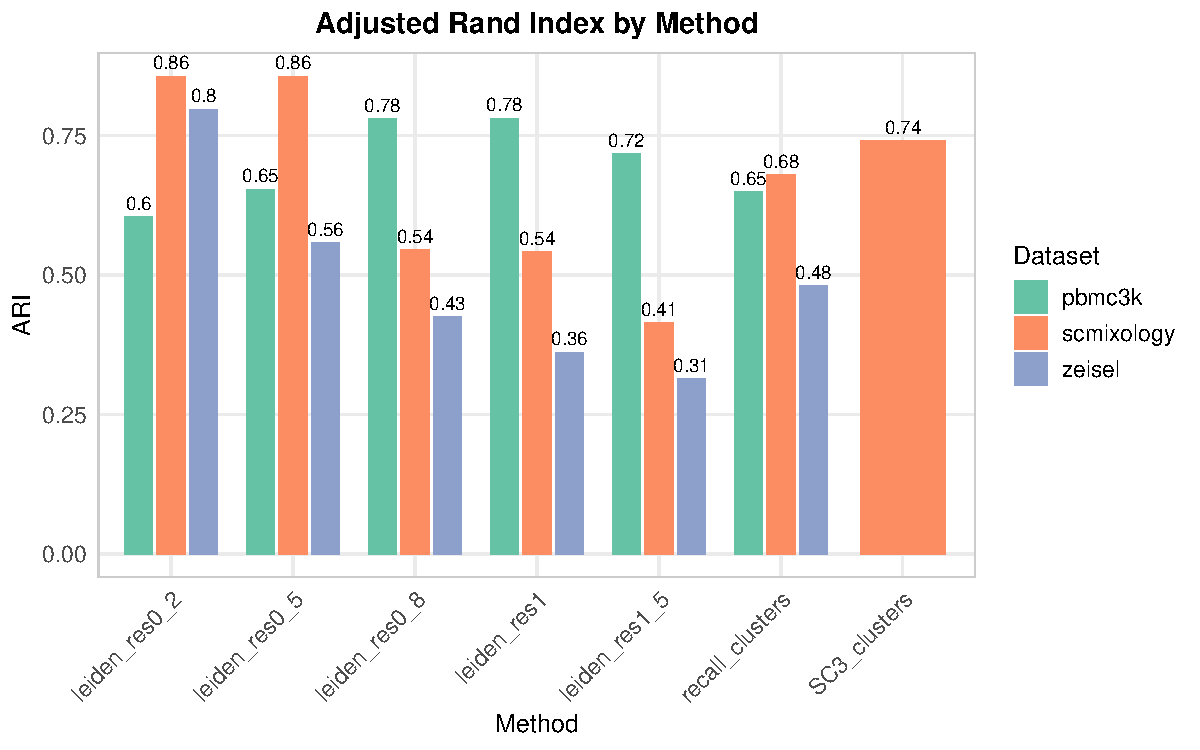
\includegraphics[width=0.9\textwidth]{figures/ari_comparison.pdf}
\caption{Adjusted Rand Index (ARI) comparison across methods and datasets. Higher values indicate better agreement with ground truth labels. Leiden results shown for multiple resolution values (0.2, 0.5, 0.8, 1.0, 1.5). SC3 results available only for scMixology. The optimal resolution varies by dataset: scMixology and Zeisel favor low resolution, while PBMC 3k favors moderate resolution.}
\label{fig:ari_comparison}
\end{figure}

\subsection{PBMC 3k Dataset: Immune Cell Complexity}

The PBMC 3k dataset presents greater complexity with nine distinct immune cell types. Here, moderate resolution Leiden clustering (0.8--1.0) achieved the best performance (ARI = 0.781), correctly identifying eight of nine cell types. The slightly negative OCI ($-$0.11) indicates minor underclustering, with one cell type likely merged with a similar population.

recall achieved ARI = 0.649 with seven predicted clusters, reflecting its conservative merging behavior. The FDR control mechanism merged clusters that did not meet the significance threshold, resulting in underclustering relative to the ground truth (Figure~\ref{fig:nmi_comparison}).

\begin{figure}[htbp]
\centering
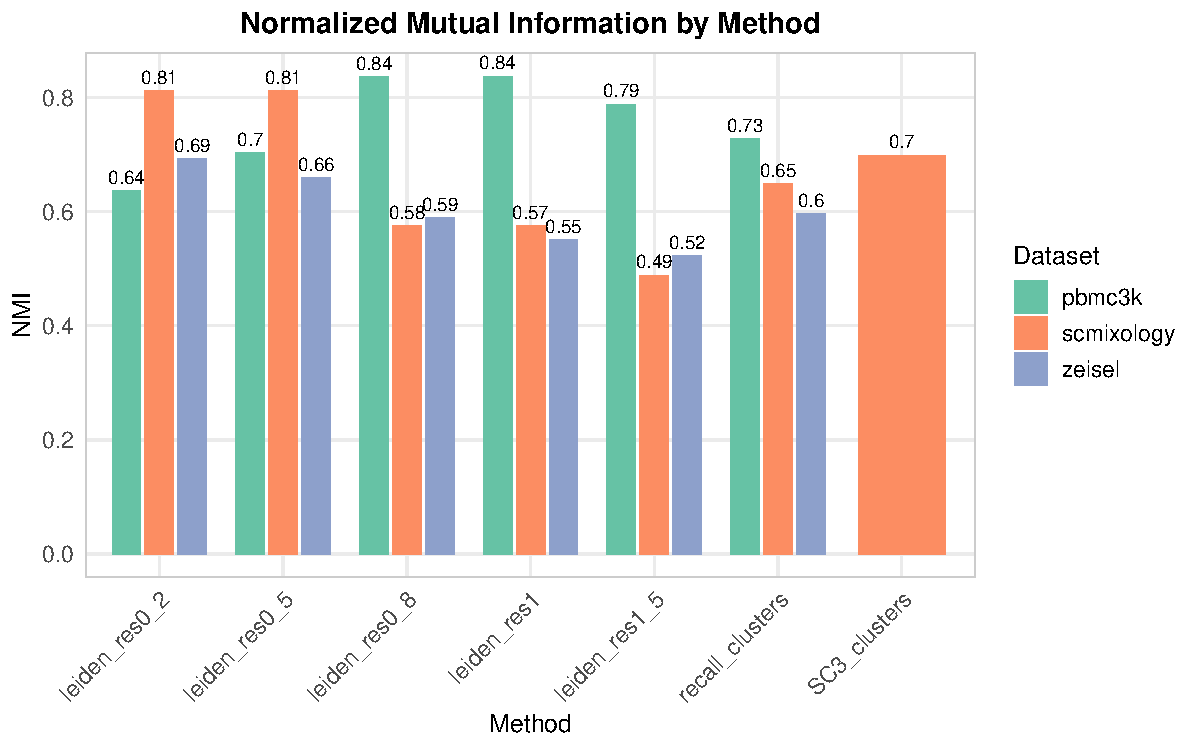
\includegraphics[width=0.9\textwidth]{figures/nmi_comparison.pdf}
\caption{Normalized Mutual Information (NMI) comparison across methods and datasets. NMI values correlate strongly with ARI but provide an information-theoretic perspective on clustering quality. Higher values indicate greater shared information between predicted and true cluster labels.}
\label{fig:nmi_comparison}
\end{figure}

\subsection{Zeisel Brain Dataset: Hierarchical Structure}

The Zeisel dataset, with its hierarchical structure of neuronal and glial cell types, revealed an interesting pattern. Low-resolution Leiden (0.2) achieved the highest ARI (0.797) despite identifying only four clusters versus the true seven. This counterintuitive result suggests that the level1 annotation may not represent the optimal clustering granularity for this dataset---the four predicted clusters may correspond to biologically meaningful groupings at a coarser level.

Higher resolution values that matched the ground truth cluster count ($K=7$ at resolution 0.8) achieved lower ARI (0.425), indicating that forcing the correct number of clusters does not guarantee correct cluster assignments. recall achieved ARI = 0.481 with eight predicted clusters.

\subsection{Cluster Count Analysis}

Figure~\ref{fig:cluster_counts} illustrates the relationship between resolution parameter and predicted cluster count across datasets. As expected, cluster count increases monotonically with resolution for Leiden clustering. The ground truth cluster count is indicated for reference.

\begin{figure}[htbp]
\centering
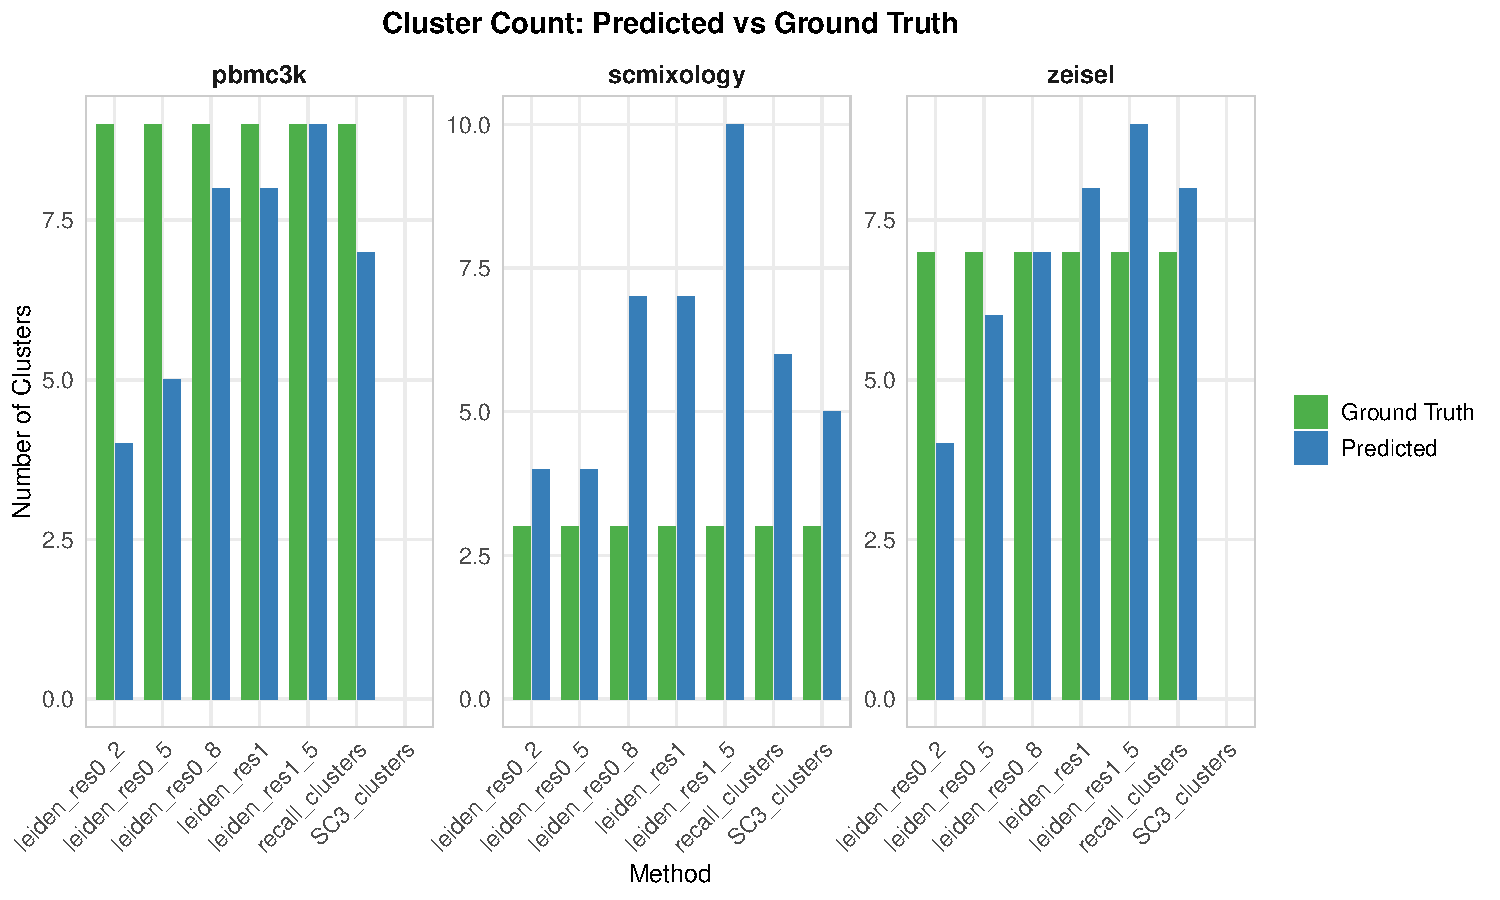
\includegraphics[width=0.85\textwidth]{figures/cluster_counts.pdf}
\caption{Number of clusters identified by each method across datasets. Horizontal dashed lines indicate ground truth cluster counts (scMixology: 3, PBMC 3k: 9, Zeisel: 7). Leiden cluster counts increase with resolution. SC3 and recall provide single predictions per dataset without resolution tuning.}
\label{fig:cluster_counts}
\end{figure}

\subsection{Overclustering Analysis}

The overclustering index (OCI) quantifies the tendency of methods to over- or under-partition the data (Figure~\ref{fig:overclustering}). For scMixology, all methods exhibited positive OCI, with Leiden at resolution 1.5 showing the most severe overclustering (OCI = 2.33, corresponding to 10 clusters vs. 3 true). For PBMC 3k, moderate underclustering was observed across methods. For Zeisel, low-resolution Leiden substantially underclustered (OCI = $-$0.43), while higher resolutions approached the ground truth count.

\begin{figure}[htbp]
\centering
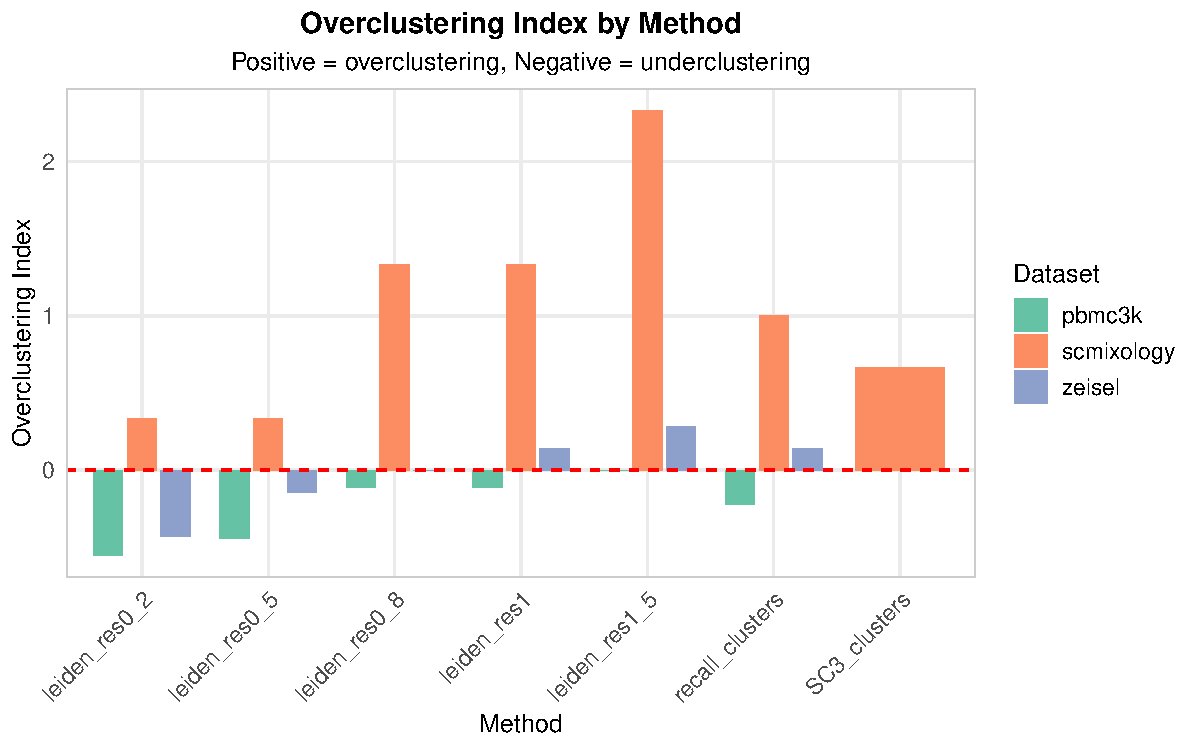
\includegraphics[width=0.85\textwidth]{figures/overclustering_analysis.pdf}
\caption{Overclustering Index (OCI) by method and dataset. OCI = $(K_{\text{predicted}} - K_{\text{true}}) / K_{\text{true}}$. Positive values indicate overclustering; negative values indicate underclustering; zero indicates exact cluster count match. Statistical calibration methods (SC3, recall) show varying behavior depending on dataset complexity.}
\label{fig:overclustering}
\end{figure}

\subsection{UMAP Visualization}

UMAP~\cite{mcinnes2018umap} visualizations provide qualitative assessment of clustering quality. Figure~\ref{fig:umap_scmixology} shows the scMixology results, where the three cell lines form clearly separated clusters. Leiden at low resolution correctly identifies these populations, while higher resolutions fragment them into multiple clusters.

\begin{figure}[htbp]
\centering
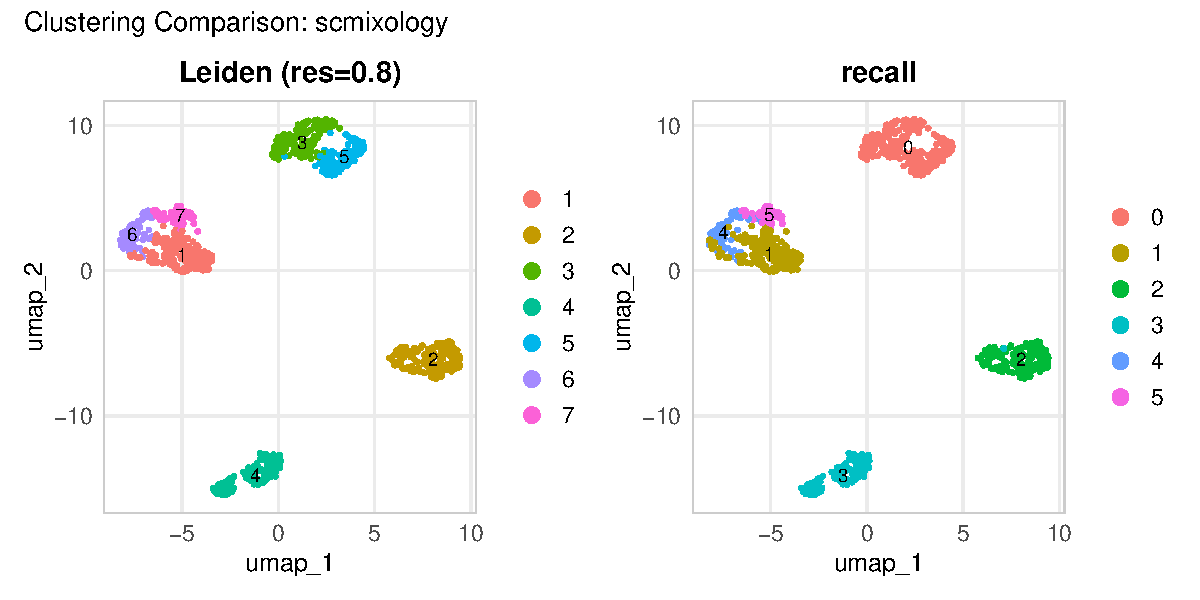
\includegraphics[width=0.9\textwidth]{figures/umap_scmixology.pdf}
\caption{UMAP visualization of scMixology clustering results. The three cell lines (HCC827, H1975, H2228) form well-separated clusters in the embedding space. Panel A shows ground truth labels; subsequent panels show predicted clusters from different methods. Color coding indicates cluster assignment.}
\label{fig:umap_scmixology}
\end{figure}

The PBMC 3k and Zeisel datasets show more complex structure with overlapping populations (Figures~\ref{fig:umap_pbmc3k} and~\ref{fig:umap_zeisel}), explaining the greater challenge in achieving high clustering accuracy.

\begin{figure}[htbp]
\centering
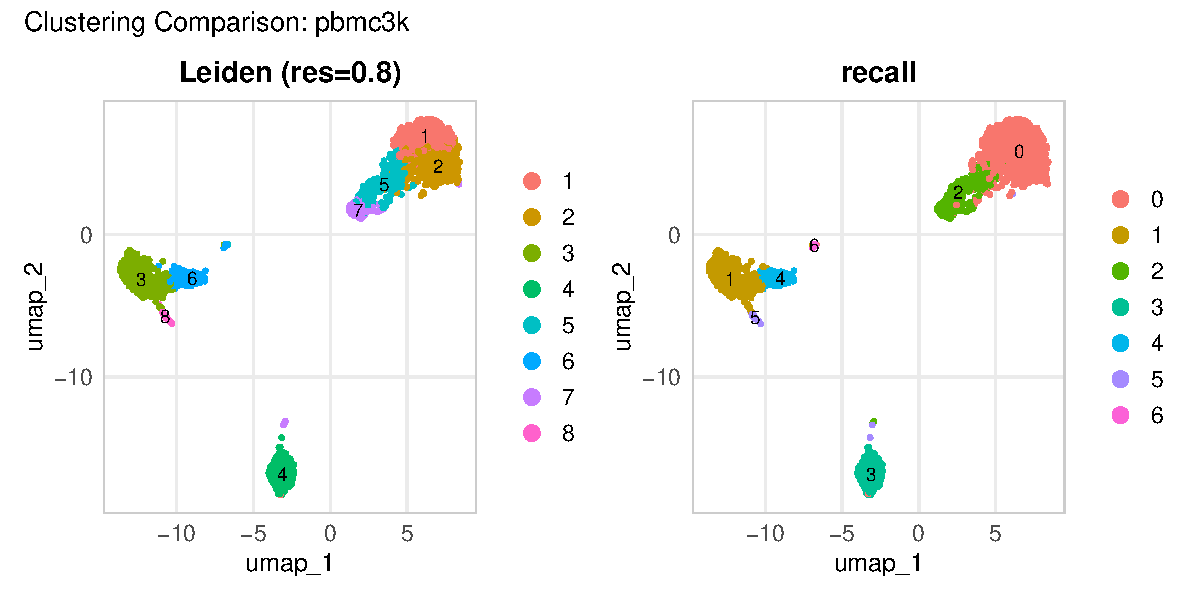
\includegraphics[width=0.9\textwidth]{figures/umap_pbmc3k.pdf}
\caption{UMAP visualization of PBMC 3k clustering results. Nine immune cell types show varying degrees of separation, with some populations (e.g., CD4+ and CD8+ T-cells) exhibiting overlapping expression profiles. Monocyte and NK cell populations are well separated.}
\label{fig:umap_pbmc3k}
\end{figure}

\begin{figure}[htbp]
\centering
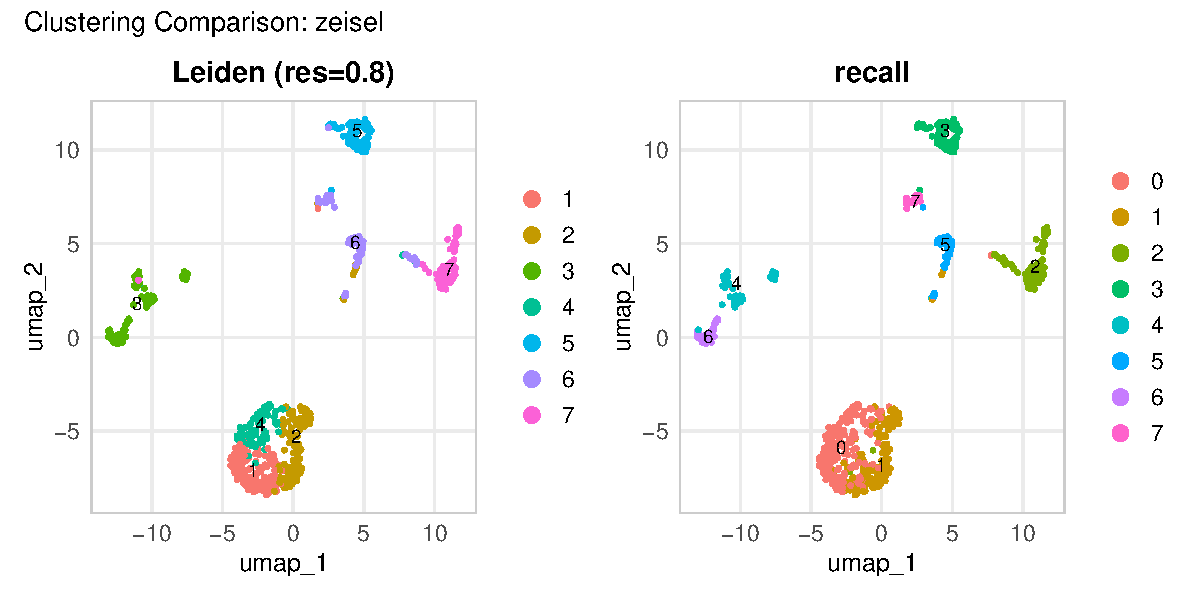
\includegraphics[width=0.9\textwidth]{figures/umap_zeisel.pdf}
\caption{UMAP visualization of Zeisel brain dataset clustering results. Seven major cell classes at the level1 annotation show hierarchical structure, with neuronal and glial populations occupying distinct regions of the embedding space.}
\label{fig:umap_zeisel}
\end{figure}

\subsection{Extended Metrics}

Table~\ref{tab:extended_metrics} presents the complete set of clustering metrics for all methods and datasets.

\begin{table}[htbp]
\centering
\caption{Extended clustering metrics for all methods. Homog.: Homogeneity; Compl.: Completeness; Silh.: Silhouette Score.}
\label{tab:extended_metrics}
\small
\begin{tabular}{@{}llcccccc@{}}
\toprule
\textbf{Dataset} & \textbf{Method} & \textbf{K} & \textbf{ARI} & \textbf{NMI} & \textbf{Homog.} & \textbf{Compl.} & \textbf{Silh.} \\
\midrule
\multirow{7}{*}{scMixology}
    & Leiden 0.2 & 4 & 0.856 & 0.812 & 0.987 & 0.812 & 0.354 \\
    & Leiden 0.5 & 4 & 0.856 & 0.812 & 0.987 & 0.812 & 0.354 \\
    & Leiden 0.8 & 7 & 0.545 & 0.576 & 0.988 & 0.576 & 0.212 \\
    & Leiden 1.0 & 7 & 0.542 & 0.575 & 0.988 & 0.575 & 0.211 \\
    & Leiden 1.5 & 10 & 0.415 & 0.489 & 0.989 & 0.489 & 0.178 \\
    & SC3 & 5 & 0.741 & 0.699 & 0.982 & 0.699 & 0.268 \\
    & recall & 6 & 0.680 & 0.649 & 0.982 & 0.649 & 0.290 \\
\midrule
\multirow{6}{*}{PBMC 3k}
    & Leiden 0.2 & 4 & 0.604 & 0.637 & 0.637 & 0.948 & 0.232 \\
    & Leiden 0.5 & 5 & 0.654 & 0.703 & 0.703 & 0.935 & 0.231 \\
    & Leiden 0.8 & 8 & 0.780 & 0.836 & 0.836 & 0.838 & 0.128 \\
    & Leiden 1.0 & 8 & 0.781 & 0.837 & 0.837 & 0.838 & 0.128 \\
    & Leiden 1.5 & 9 & 0.717 & 0.788 & 0.843 & 0.788 & 0.102 \\
    & recall & 7 & 0.649 & 0.728 & 0.728 & 0.935 & 0.236 \\
\midrule
\multirow{6}{*}{Zeisel}
    & Leiden 0.2 & 4 & 0.797 & 0.692 & 0.692 & 0.819 & 0.315 \\
    & Leiden 0.5 & 6 & 0.558 & 0.660 & 0.781 & 0.660 & 0.183 \\
    & Leiden 0.8 & 7 & 0.425 & 0.590 & 0.785 & 0.590 & 0.128 \\
    & Leiden 1.0 & 8 & 0.362 & 0.551 & 0.787 & 0.551 & 0.110 \\
    & Leiden 1.5 & 9 & 0.315 & 0.523 & 0.791 & 0.524 & 0.095 \\
    & recall & 8 & 0.481 & 0.597 & 0.790 & 0.597 & 0.140 \\
\bottomrule
\end{tabular}
\end{table}

Notable observations from the extended metrics:
\begin{itemize}[noitemsep]
    \item \textbf{Homogeneity} remains high ($>0.98$) for scMixology across all methods, indicating that predicted clusters consistently contain cells from the same true population
    \item \textbf{Completeness} decreases with increasing resolution, as overclustering splits true populations across multiple predicted clusters
    \item \textbf{Silhouette scores} decrease with higher resolution, reflecting less well-defined cluster boundaries when data is over-partitioned
\end{itemize}

% =============================================================================
% 05_discussion.tex - Discussion
% =============================================================================

\section{Discussion}
\label{sec:discussion}

\subsection{Key Findings}

Our comparative analysis of three clustering approaches---Seurat/Leiden, SC3, and recall---reveals several important insights for the scRNA-seq community:

\begin{enumerate}
    \item \textbf{No single method dominates across all datasets}: Leiden clustering achieved the best ARI on all three datasets, but the optimal resolution varied substantially (0.2 for scMixology and Zeisel, 1.0 for PBMC 3k). This underscores the fundamental challenge of resolution selection in graph-based clustering.

    \item \textbf{Optimal resolution correlates with dataset complexity}: Simpler datasets with well-separated populations (scMixology) perform best at low resolution, while complex datasets with many similar populations (PBMC 3k) require higher resolution to distinguish subtypes.

    \item \textbf{Consensus clustering provides stability but not scalability}: SC3 achieved competitive accuracy (ARI = 0.741) on scMixology through its ensemble approach, but memory constraints prevented application to larger datasets. This represents a significant limitation for modern single-cell experiments that routinely generate tens of thousands of cells.

    \item \textbf{FDR control may be overly conservative}: recall's knockoff-based approach consistently underestimated cluster count relative to ground truth, suggesting that the FDR threshold (q = 0.05) may be too stringent for some biological applications. Adjusting this threshold could improve sensitivity at the cost of potentially increased false discoveries.
\end{enumerate}

\subsection{Resolution Selection Paradox}

A striking finding from this study is that matching the ground truth cluster count does not guarantee high clustering accuracy. On the Zeisel dataset, Leiden at resolution 0.8 produced exactly seven clusters (matching the ground truth), yet achieved only ARI = 0.425. In contrast, resolution 0.2 produced only four clusters but achieved ARI = 0.797.

This paradox arises because ARI measures the agreement of pairwise cell assignments, not cluster count. A clustering that correctly groups cells into four coarse categories can achieve higher ARI than one that attempts seven categories but assigns many cells incorrectly. This finding has implications for how researchers should interpret ground truth annotations---particularly for datasets with hierarchical structure, the ``correct'' number of clusters may be ambiguous.

\subsection{Future Directions}

Several promising directions emerge from this work:

\begin{itemize}[noitemsep]
    \item \textbf{Adaptive FDR thresholds}: Developing methods to select appropriate FDR thresholds based on dataset characteristics could improve recall's sensitivity

    \item \textbf{Scalable consensus clustering}: Memory-efficient implementations of SC3 or alternative consensus approaches could extend its applicability to larger datasets

    \item \textbf{Integration with foundation models}: Pre-trained embeddings from models like scGPT or GeneCompass may provide more informative representations for clustering

    \item \textbf{Multi-resolution integration}: Methods that combine information across multiple resolution scales could provide more robust clustering without requiring resolution selection

    \item \textbf{Benchmarking on additional datasets}: Extending this comparison to additional datasets with different characteristics (e.g., developmental trajectories, disease states) would strengthen the generalizability of our recommendations
\end{itemize}

% =============================================================================
% 06_conclusion.tex - Conclusion
% =============================================================================

\section{Conclusion}
\label{sec:conclusion}

This study presents a systematic comparison of three clustering approaches for single-cell RNA sequencing data: Seurat/Leiden graph-based clustering, SC3 consensus clustering, and recall FDR-controlled clustering. Our analysis of three benchmark datasets with known ground truth yields the following conclusions:

\begin{enumerate}
    \item \textbf{Leiden clustering remains competitive but requires resolution selection}: Standard Leiden clustering achieved the highest ARI across all datasets when the resolution parameter was appropriately tuned. However, the optimal resolution varied substantially across datasets (0.2 for scMixology and Zeisel, 1.0 for PBMC 3k), highlighting the challenge of parameter selection without ground truth.

    \item \textbf{SC3 provides robust clustering for small datasets}: SC3's consensus approach achieved strong performance (ARI = 0.741) on the scMixology dataset, demonstrating the value of ensemble methods. However, its $O(n^2)$ memory complexity limits applicability to datasets with fewer than approximately 1,000 cells.

    \item \textbf{recall provides statistical rigor at the cost of sensitivity}: The recall method's FDR control mechanism provides principled cluster validation, addressing the double-dipping problem that afflicts uncalibrated clustering. However, its conservative merging behavior may underestimate true cluster count in some biological contexts.

    \item \textbf{Matching cluster count does not guarantee accuracy}: Our results demonstrate that producing the ``correct'' number of clusters does not ensure high clustering accuracy, particularly for datasets with hierarchical structure. Evaluation should focus on cell-level agreement (ARI, NMI) rather than cluster count alone.

    \item \textbf{No single method dominates}: The optimal clustering approach depends on dataset characteristics, computational resources, and analytical goals. We provide guidelines to assist researchers in method selection.
\end{enumerate}

We recommend that researchers adopt a multi-method approach: use Leiden clustering at multiple resolutions for exploratory analysis, apply recall for statistical validation of cluster significance, and consider SC3 for small datasets where memory is not limiting. The field would benefit from continued development of methods that combine the scalability of graph-based approaches with the statistical rigor of calibration methods.

\subsection*{Data Availability}

All code, data processing scripts, and analysis pipelines are available at \url{https://github.com/adrianstanea/scRNA-seq-Clustering}. Processed datasets and clustering results are provided for reproducibility.

\subsection*{Acknowledgments}

We thank the developers of Seurat, SC3, and recall for making their methods freely available. We acknowledge the original authors of the benchmark datasets: Tian et al. for scMixology, 10x Genomics for PBMC 3k, and Zeisel et al. for the mouse brain dataset.



\newpage
% Bibliography
\bibliographystyle{unsrtnat}
\bibliography{bibliography/references}

% % Appendix
% \appendix
% % =============================================================================
% 07_appendix.tex - Appendix
% =============================================================================

\section{Supplementary Materials}
\label{sec:appendix}

\subsection{Environment Configuration}

\subsubsection{R Environment}

\begin{lstlisting}[language=R, caption={R package versions used in this study}]
# Core packages
R version 4.3.x
Seurat >= 5.0.0
SC3 >= 1.28.0  # Bioconductor
recall >= 0.1.0
ggplot2 >= 3.4.0
dplyr >= 1.1.0

# Installation commands
# Seurat
install.packages("Seurat")

# SC3 (Bioconductor)
BiocManager::install("SC3")

# recall (GitHub)
devtools::install_github("lcrawlab/recall")
\end{lstlisting}

\subsubsection{Python Environment}

\begin{lstlisting}[language=Python, caption={Python package versions for complementary analysis}]
# environment.yml
python >= 3.10
scanpy >= 1.10
anndata >= 0.10
scikit-learn >= 1.3
matplotlib >= 3.7
pandas >= 2.0
numpy >= 1.24
\end{lstlisting}

\subsection{Parameter Configurations}

\subsubsection{Preprocessing Parameters}

\begin{lstlisting}[caption={preprocessing\_params.yaml}]
qc:
  min_genes_per_cell: 200
  max_genes_per_cell: 5000
  max_pct_mt: 5.0
  min_cells_per_gene: 3

normalization:
  method: "LogNormalize"
  scale_factor: 10000

feature_selection:
  method: "vst"
  n_top_genes: 2000

dimensionality_reduction:
  n_pcs: 30
  n_neighbors: 20

random_seed: 42
\end{lstlisting}

\subsubsection{Clustering Parameters}

\begin{lstlisting}[caption={clustering\_params.yaml}]
leiden:
  resolutions: [0.2, 0.5, 0.8, 1.0, 1.5]
  algorithm: "leiden"
  n_iterations: -1  # Run until convergence

sc3:
  # Automatic k estimation via Tracy-Widom test
  estimate_k: true
  # If manual, specify range
  k_range: [2, 10]
  # Distance metrics
  distances: ["euclidean", "pearson", "spearman"]
  # Transformations
  transformations: ["pca", "laplacian"]
  # Number of k-means runs per configuration
  n_runs: 5

recall:
  reduction: "pca"
  dims: 30
  fdr: 0.05
  method: "leiden"
  n_knockoffs: 1

evaluation:
  metrics:
    - "ARI"
    - "NMI"
    - "Silhouette"
    - "Homogeneity"
    - "Completeness"

random_seed: 42
\end{lstlisting}

\subsection{Complete Metrics by Dataset}

\subsubsection{scMixology Dataset}

\begin{table}[htbp]
\centering
\caption{Complete clustering metrics for scMixology dataset (902 cells, 3 ground truth clusters).}
\label{tab:scmixology_full}
\small
\begin{tabular}{@{}lcccccc@{}}
\toprule
\textbf{Method} & \textbf{K} & \textbf{ARI} & \textbf{NMI} & \textbf{Homog.} & \textbf{Compl.} & \textbf{Silh.} \\
\midrule
Leiden res=0.2 & 4 & 0.856 & 0.812 & 0.987 & 0.812 & 0.354 \\
Leiden res=0.5 & 4 & 0.856 & 0.812 & 0.987 & 0.812 & 0.354 \\
Leiden res=0.8 & 7 & 0.545 & 0.576 & 0.988 & 0.576 & 0.212 \\
Leiden res=1.0 & 7 & 0.542 & 0.575 & 0.988 & 0.575 & 0.211 \\
Leiden res=1.5 & 10 & 0.415 & 0.489 & 0.989 & 0.489 & 0.178 \\
SC3 & 5 & 0.741 & 0.699 & 0.982 & 0.699 & 0.268 \\
recall & 6 & 0.680 & 0.649 & 0.982 & 0.649 & 0.290 \\
\bottomrule
\end{tabular}
\end{table}

\subsubsection{PBMC 3k Dataset}

\begin{table}[htbp]
\centering
\caption{Complete clustering metrics for PBMC 3k dataset (2,643 cells, 9 ground truth clusters).}
\label{tab:pbmc3k_full}
\small
\begin{tabular}{@{}lcccccc@{}}
\toprule
\textbf{Method} & \textbf{K} & \textbf{ARI} & \textbf{NMI} & \textbf{Homog.} & \textbf{Compl.} & \textbf{Silh.} \\
\midrule
Leiden res=0.2 & 4 & 0.604 & 0.637 & 0.637 & 0.948 & 0.232 \\
Leiden res=0.5 & 5 & 0.654 & 0.703 & 0.703 & 0.935 & 0.231 \\
Leiden res=0.8 & 8 & 0.780 & 0.836 & 0.836 & 0.838 & 0.128 \\
Leiden res=1.0 & 8 & 0.781 & 0.837 & 0.837 & 0.838 & 0.128 \\
Leiden res=1.5 & 9 & 0.717 & 0.788 & 0.843 & 0.788 & 0.102 \\
recall & 7 & 0.649 & 0.728 & 0.728 & 0.935 & 0.236 \\
\bottomrule
\end{tabular}
\end{table}

\subsubsection{Zeisel Brain Dataset}

\begin{table}[htbp]
\centering
\caption{Complete clustering metrics for Zeisel brain dataset (680 cells, 7 ground truth clusters at level1).}
\label{tab:zeisel_full}
\small
\begin{tabular}{@{}lcccccc@{}}
\toprule
\textbf{Method} & \textbf{K} & \textbf{ARI} & \textbf{NMI} & \textbf{Homog.} & \textbf{Compl.} & \textbf{Silh.} \\
\midrule
Leiden res=0.2 & 4 & 0.797 & 0.692 & 0.692 & 0.819 & 0.315 \\
Leiden res=0.5 & 6 & 0.558 & 0.660 & 0.781 & 0.660 & 0.183 \\
Leiden res=0.8 & 7 & 0.425 & 0.590 & 0.785 & 0.590 & 0.128 \\
Leiden res=1.0 & 8 & 0.362 & 0.551 & 0.787 & 0.551 & 0.110 \\
Leiden res=1.5 & 9 & 0.315 & 0.523 & 0.791 & 0.524 & 0.095 \\
recall & 8 & 0.481 & 0.597 & 0.790 & 0.597 & 0.140 \\
\bottomrule
\end{tabular}
\end{table}

\subsection{Technical Issues Encountered}

\subsubsection{CHOIR Dependency Conflict}

CHOIR~\cite{sant2025choir} was initially planned for inclusion in this comparative study. However, the package could not be installed due to a dependency conflict in Bioconductor 3.19:

\begin{lstlisting}[caption={CHOIR installation error}]
Error: package 'treeio' was installed before R 4.4.0
Error: package 'yulab.utils' version mismatch
\end{lstlisting}

These packages are required for CHOIR's hierarchical tree visualization functionality. Future work should revisit CHOIR once these dependency issues are resolved in subsequent Bioconductor releases.

\subsubsection{SC3 Memory Constraints}

SC3's consensus matrix construction requires storing pairwise cell similarities, resulting in $O(n^2)$ memory complexity:

\begin{equation}
\text{Memory (bytes)} \approx 8 \times n^2
\end{equation}

For the PBMC 3k dataset ($n = 2643$), this requires approximately 56 MB for the consensus matrix alone. Combined with intermediate computations and multiple distance metrics, total memory requirements exceeded available RAM (16 GB) during analysis. The scMixology dataset ($n = 902$) required approximately 6.5 MB and completed successfully.

\subsection{Computational Environment}

All experiments were conducted on the following system:
\begin{itemize}[noitemsep]
    \item Operating System: Linux (Ubuntu 22.04 via WSL2)
    \item Kernel: 6.6.87.2-microsoft-standard-WSL2
    \item R Version: 4.3.x with Seurat 5.x
    \item Python Version: 3.10+ with Scanpy 1.10+
    \item RAM: 16 GB
    \item Storage: SSD
\end{itemize}

\subsection{Reproducibility Checklist}

To reproduce the results presented in this study:

\begin{enumerate}[noitemsep]
    \item Clone the repository: \texttt{git clone https://github.com/adrianstanea/scRNA-seq-Clustering}
    \item Install R dependencies: \texttt{renv::restore()}
    \item Download datasets: Run \texttt{src/R/01\_download\_data.R}
    \item Preprocess data: Run \texttt{src/R/02\_preprocessing.R}
    \item Run Leiden clustering: Run \texttt{src/R/03\_leiden\_clustering.R}
    \item Run SC3 clustering: Run \texttt{src/R/04\_sc3\_clustering.R}
    \item Run recall clustering: Run \texttt{src/R/05\_recall\_clustering.R}
    \item Compute metrics: Run \texttt{src/R/06\_evaluation.R}
    \item Generate figures: Run \texttt{src/R/07\_visualization.R}
\end{enumerate}

All scripts use random seed 42 for reproducibility. Expected runtime on the specified hardware is approximately 30 minutes for the complete pipeline.


\end{document}
